% !TeX document-id = {beb7ced9-b3cd-42b2-b16a-3ed3c633a1d9}
\documentclass[]             % options: RDPonly, coveronly, nocover
{NASA}                       %   plus standard article class options
%\DeclareRobustCommand{\mmodels}{\mathrel{|}\joinrel\Relbar}

\usepackage[utf8]{inputenc}
\usepackage{csquotes}
\usepackage{setspace}
\usepackage{hyperref}
\usepackage{amsmath, amssymb, amscd, amsthm, amsfonts}
\usepackage{mathtools}
\usepackage{graphicx}
\usepackage{hyperref}
\usepackage{amsthm}
\usepackage[english]{babel}
\usepackage{proof}

\newtheorem{example}{Example}

\newcommand{\B}{\mathbf{B}}
\newcommand{\w}{\mathbf{w}}
\usepackage{proof}
\usepackage{tikz-cd}
\tikzcdset{scale cd/.style={every label/.append style={scale=#1},
		cells={nodes={scale=#1}}}}
\usepackage{stmaryrd}
\hypersetup{
	colorlinks=true,
	linkcolor=blue,
	filecolor=magenta,
	urlcolor=cyan,
	pdftitle={Overleaf Example},
	pdfpagemode=FullScreen,
}
\urlstyle{same}

\newtheorem{theorem}{Theorem}[section]
\newtheorem{corollary}{Corollary}[theorem]
\newtheorem{lemma}[theorem]{Lemma}

\theoremstyle{definition}
\newtheorem{definition}{Definition}[section]

\title{An Analysis of Distributed Computing Challenges in Coordinating
  Airborne and Ground-Based Agents} \author{Lawrence Dunn and Alwyn
  E. Goodloe}

\AuthorAffiliation{Lawrence Dunn \\ Department of Computer and Information
Science \\ University of Pennsylvania \\ Philadelphia, PA \\ Alwyn Goodloe\\                                          % for cover page
  NASA Langley Research Center, Hampton, Virginia
}
\NasaCenter{Langley Research Center\\Hampton, Virginia 23681-2199}
\Type{TM}                    % TM, TP, CR, CP, SP, TT
\SubjectCategory{64}         % two digit number
\LNumber{XXXXX}              % Langley L-number
\Number{XXXXXX}              % Report number
\Month{12}                   % two digit number
\Year{2022}                  % four digit number
\SubjectTerms{Distributed Systems, Formal Methods, Logic, }     % 4-5 comma separated words
\Pages{46}                   % all the pages from the front to back covers
\DatesCovered{}              % 10/2000--9/2002
\ContractNumber{}            % NAS1-12345
\GrantNumber{}               % NAG1-1234
\ProgramElementNumber{}
\ProjectNumber{}             % NCC1-123
\TaskNumber{}                % Task 123
\WorkUnitNumber{}            % 123-45-67-89
\SupplementaryNotes{}
\Acknowledgment{The work was conducted during a summer internship at the NASA Langley Research Center in the Safety-Critical Avionics Systems Branch focusing on distributed computing  issues arising in the Safety Demonstrator challenge in the NASA Aeronautics System Wide Safety (SWS) program.}

\abstract{TBD}

\begin{document}
\newpage
\setcounter{tocdepth}{2}
\tableofcontents
\newpage
\section{Introduction}
Civil aviation has primarily been focused on efficiently moving goods
and people via the airspace to their destination. The application of
sound engineering practices and conservative operating procedures has
made flying the safest mode of transport. Now the desire not to
compromise this safety makes it challenging to introduce uncrewed
vehicles into the airspace. The rules for operating in the US national
airspace are typically relaxed during natural disasters and relief
efforts, however. The NASA Aeronautics' Airspace Operations and Safety
Program (AOSP) System Wide Safety (SWS) project has been investigating
how crewed and uncrewed aircraft may safely operate in shared
airspace, taking wildfire fighting and hurricane relief as use cases.

Disaster response scenarios like the ones under consideration present
unique challenges for safe operations, particularly because of the
unpredictable communications environment combined with the need for
system-wide coordination. Traditionally, civil aviation has employed
simple communication patterns between air and ground and among
aircraft. A typical airborne protocol is Automatic Dependent
Surveillance-Broadcast (ADS-B), by which aircraft periodically
broadcast their position and velocity to air traffic controllers and
nearby aircraft. The use cases under consideration demand more
sophisticated coordination between airborne and ground-based elements
to accomplish mission goals such as navigating safely in close
proximity, delivering resources, and fighting fires. However, the
operating environment will not admit the use of reliable,
high-bandwidth internet connections that consistently allow clients to
transmit large amounts of data quickly. For instance, obstructions
like distance, terrain, smoke, and weather mean we should expect
network packets to be dropped or delayed in unpredictable
ways. Therefore, network performance will be relatively difficult to
predict and control.

An unreliable communications environment makes it difficult to
coordinate agents and offer strong safety guarantees. This is a
challenge of distributed computing, a subdiscipline of computer
science. This purpose of this memorandum is to enumerate some of the
considerations involved in coordinating air- and ground-based elements
from a distributed computing perspective, identifying challenges,
potential requirements, and frameworks that may aid in developing
solutions.

The rest of this document is laid out as follows. Section 2 provides a
high-level introduction to the challenges of distributed computing,
focusing on Brewer's CAP theorem that captures the
consistency/availability (C/A) tradeoff in the presense of network
partitions (P). We offer a list of three desiderata of distributed
applications in the contexts under consideration.  Section 3 explains
how the framework of \emph{conits} \cite{} may be used for quantifying
the nature of the C/A tradeoff in the context of data replication, a
desirable feature for safety-critical systems. Section 4 is an
introduction to applied sheaf theory, which provides a highly general
framework for measuring the mutual consistency of ``overlapping''
observations (i.e. ones which we expect to be correlated if not equal,
such as the data generated by a sensor network). We discuss an
simulated example, due to \cite{}, where sheaves are used to integrate
heterogeneous sensor data, thereby improving an estimated location for
a crashed aircraft. Section 5 is a conclusion with suggestions for
future work.

\section{Consistency in distributed systems}
\label{sec:distrsys}

A distributed system, broadly construed, is a collection of
independent entities that cooperate to solve a problem that cannot be
individually solved \cite{kshemkalyani_singhal_2008}. Here we are
concerned with the sorts of distributed systems involved in civil
aviation in the context of disaster response scenarios like combating
wildfires and providing hurricane relief. In these scenarios, entities
like emergency responders, firefighters, crewed and uncrewed aircraft
teams, air traffic controllers, and other personnel cooperate to solve
shared tasks like navigating safely, delivering resources,
extinguishing fires, and collecting and sharing data. A paramount
concern in all of our use cases is that the system must ensure strong
safety guarantees.

Safely coordinating the actions of distributed agents is a challenge
for distributed computing. Singhal and Shivaratri
\cite{10.5555/562065} characterized a distributed computing system as
\begin{quotation}
  A collection of computers that do not share common memory or a
  common physical clock, that communicate by message passing over a
  communication network, and where each computer has its own memory
  and runs its own operating system.
\end{quotation}
``Computers" here should be understood broadly, taken to include
aircraft systems like ADS-B, portable communications equipment,
satellites, vehicle-mounted personal computers, or smartphones carried
by firefighters in the field.

Absence of a common memory implies that all communication between
system nodes takes place over the network, rather than by writing data
to mutually accessible memory. In general, and particularly during
disaster response scenarios, message delivery is neither guaranteed
nor instantaneous. For example, two firefighting ground teams may not
be able to communicate with each other over a radio network if the
teams are separated by a tall ridgeline. Handling these sorts of
challenges gracefully---for example, automatically redirecting a
nearby drone to route messages over the ridgeline---requires
sophisticated distributed applications that can tolerate a chaotic
operating environment and network.

A highly centralized network topology relying on a small number of
central nodes to route messages and coordinate betwee nodes would be
too brittle for our intended use cases. Such a setup could allow, for
instance, the failure of a centrally-located node to wreak havoc on
the rest of the system, potentially even triggering cascading
failures. Instead our model is that ground-based and airborne agents
interact as clients over an ad-hoc mesh-style network, say one
supported by the deployment of portable communication towers. We
imagine that messages are routed in a somewhat or entirely
decentralized, peer-to-peer fashion, as such a setup would be more
more resilient to the challenges of an unpredictable
environment. Compared to, say, a datacenter's fiber-optic local area
network, there are fewer guarantees about how reliably messages can be
transmitted between any two clients.

As manifest in results like Brewer's CAP theorem, below, the
imperfections in network impose theoretical and practical limitations
to how well one can coordinate distributed agents. To discuss this
topic more formally, we turn to the topic of consistency among
replicas of data objects.

\subsection{Strong consistency models}

The basic challenge of a distributed computing system is to provide
the illusion that many computers act ``as a single coherent computer''
\cite{TanenbaumSteen07} that handles the requests of every client
simultaneously. Presenting such an illusion requires coordination over
the network, so much of system coherence boils down to hiding the
effects of the unreliable network from the user.\footnote{Network
delays are a primary obstacle to coordination, but not the only
one. For instance, the fact that we do not assume nodes share
synchronized clocks makes it more challenging to enforce a global
total order of operations.}

Among the most basic distributed applications is \emph{data
replication}. In such an application, nodes maintain local replicas of
some globally shared state. For simplicity, we discuss an example
which replicates a key-value store of natural numbers, but this could
be any other kind of data structure like a FIFO queue. The application
affords clients the ability to read and/or update the data from any
node. Handling these requests requires nodes to spend time
coordinating with other nodes, e.g. to propagate updates throughout
the system, or to lookup the most up-to-date value to return to the
client. Therefore each request has a start time (when the request is
first received) and strictly greater end time (when the response is
sent back to the client). If the end time of an event $e_1$ is
strictly less than the start time of another request $e_2$, $e_1$ is
said to precede $e_2$ in external order. This gives a partial (because
some events may overlap in time) order on system events.

The figure below shows a sequence diagram of two clients interacting
with a distributed system. The vertical axis represents real
(i.e. wall-clock) time, which increases in the downward
direction. Both clients send write requests to update the natural
number associated with $x$. The reader should note that the requests
overlap in real time, with the second client's request accepted before
the first client's request has returned. After both requests are
handled, both nodes issue read requests for the same value $x$. Client
1 reads $x$ as having value $a \in \mathbb{N}$, while Client 2 reads
$b \in \mathbb{N}$.

\begin{figure}
  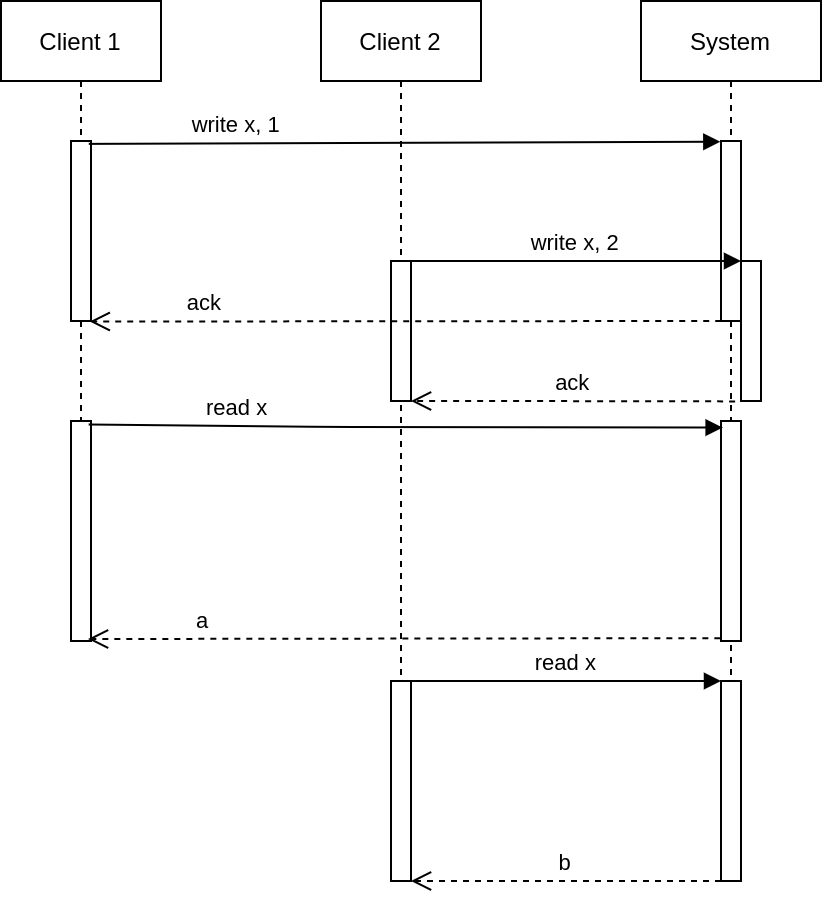
\includegraphics[scale=0.6]{Sequence Diagram.png}
  \caption{A sequence of read/write requests. A consistency model constrains the possible values of $a$ and $b$.}
\end{figure}

A \emph{consistency model} is a constraint on the allowable system
responses to these sorts of request histories. In this example, a
model constrains the possible values of $a$ and $b$. The strongest
workable consistency model is linearizability
\cite{10.1145/78969.78972}, also known as atomic
consistency.\footnote{In the context of isolated database
transactions, the analogous condition is called strict serializability
or serializability with external order.} The intuition is that to an
outside observer, a linearizable system processes requests exactly as
if they were all being handled by one node, though not always in the
order they requests were received. For instance, two consecutive read
requests must return the same value, assuming no intermediate updates
take place between the two requests. When requests are seen to
overlap, such as the updates in our example, linearizability specifies
no order on their execution. In other words, the system must act as if
during some moment while processing the request, the update instantly
took effect, but this order doesn't have to be the order in which a
request was received if they are processed concurrently.

Applied to our example, linearizability allows either write request to
take effect before the other, but they both take effect before $a$ is
read by Client 1, so $a$ must be $1$ or $2$. $b$ must have the same
value as $a$, since it is read after reading $a$ and there are no
intermediate updates to $x$. Linearizability would be violated if $b
\neq a$ because an external observer could infer the clients are
operating on different, inconsistent copies of $x$.

Enforcing linearizability imposes appreciable performance overheads on
a system, as no agent can complete an update until the update has been
propagated to all other agents. Consequently, issues with a small
number of nodes can have a disproportionately disruptive impact on the
entire application. Unsurprisingly, real-world frameworks frequently
consider models weaker than linearizability.

One weaker model, but one still regarded as a form of ``strong''
consistency, is sequential consistency
\cite{1979LamportSequential}. Here, we weaken the requirement that
effects appear to happen in an order consistent with wall clock
time. The new requirement is that the effects \emph{from a single
client} must occur in their specified order (i.e. program order), but
requests from two different clients may appear to happen in any order,
even if they don't occur concurrently in real time. Sequential
consistency would require that both $a$ and $b$ can be either 1 or 2,
with no correlation. While a real-time observer can observe behavior
that looks inconsistent with real time, the basic intuition is that if
a history is always compatible with some temporal order that
\emph{could} have happened, this is all a programmer needs to reason
about the correctness of their applications. Linearizability implies
sequential consistency, and is sometimes called sequential consistency
plus (compatibility with) external order.

Both forms of strong consistency, atomic and sequential, are too
stringent to require from many applications, especially in an
unreliable communications environment, due to performance overheads.
This phenomenon is partly captured by the so-called CAP theorem, which
we now turn to.

\subsection{The consistency/availability tradeoff}

Real-world systems often fall short of behaving as a single perfectly
coherent system. The root of this phenomenon is that there exists a
deep and well-understood tradeoff between system coherence and system
performance. Enforcing consistency comes at the cost of additional
communications, and communications impose overheads, often ones that
can be unpredictable. The network may also fail to deliver messages or
rearrange their order. Such behavior presents obstacles to
consistency, particularly if the system should also exhibit good
performance.

Fox and Brewer \cite{1999foxbrewer} observed that there is a
fundamental tension between consistency, availability, and
partition-tolerance. This tradeoff was precisely stated and proved in
2002 by Gilbert and Lynch \cite{2002gilbertlynchCAP}. To summarize
this theorem, we start by defining these terms.

\paragraph{Consistency}

Consistency in Gilbert and Lynch is defined as atomic consistency
(linearizability). The CAP theorem can be also generalized to
sequential consistency. As discussed in \cite{2019wideningcap}, this
stronger theorem is essentially already proved by Birman and Friedman
\cite{10.5555/866855}.

\paragraph{Availability}

A CAP-available system is one that will definitely respond to every
client request at some point in the future. In particular, in the
event of a network partition that prevents messages from being
delivered, the system cannot indefinitely suspend processing requests
until the network recovers, as we do not assume partitions eventually
recover. In real applications we also care about the \emph{speed} with
which requests are handled, but the CAP theorem demonstrates there are
already obstacles to ensuring that every request is handled
\emph{eventually}.

\paragraph{Partition-tolerance}

A partition tolerant system continues to function, and ensure whatever
guarantees it is meant to provide, in the face of arbitrary partitions
in the network. Note that partitions may never recover, say if a
critical communications link is permanently severed.

\begin{theorem}[CAP Theorem]
In the presense of indefinite network partitions, a distributed system
cannot guarantee both atomic consistency and availability.
\end{theorem}

The proof is not complicated. Indeed, it is almost trivial. We give
only a sketch here, leaving the interested reader to consult Gilbert
and Lynch \cite{2002gilbertlynchCAP}. In the example above, suppose the two clients have
their requests served by two different system nodes, and suppose these
nodes cannot pass messages due to an indefinite network
partition. Linearizability requires that $a$ is $1$ or $2$ and $b =
a$.  Clearly $a$ cannot be $2$ if there is no communication between
the two clients. But clearly $b$ cannot be $1$ for the same reason.
To avoid violating the condition $b = a$ we could suppose the system
indefinitely delays responding to the read requests, but this violates
our requirement that system nodes eventually respond to
clients. Therefore, $P$ implies we cannot have both $C$ and $A$.

While the proof of the CAP theorem is rather trivial, its
interpretation is subtle and has been the subject of much discussion
in the years since \cite{2012CAP12Years}. It is sometimes assumed that
the CAP theorem claims that a distributed system can only offer two of
the properties C, A, and P. In fact, the theorem constrains, but does
not prohibit the existence of, applications that apply some relaxed
amount of all three features. The CAP theorem only rules out their
combination when all three are interpreted in a highly idealized
sense.

One way the the CAP theorem is idealized is that it defines
consistency as linearizability, a very strong condition. In practice
one often tolerates weaker levels of consistency. Also, network
partitions are often not as dramatic as an indefinite total
communications blackout. Real-world conditions in our context are
likely more chaotic, featuring many smaller disruptions and delays and
sometimes larger ones. Communications between different clients may be
affected differently, with nearby agents generally likely to have
better communication channels between them than agents that are far
apart. Finally, CAP-availability is a suprisingly weak condition. It
only requires that requests are handled eventually. In a truly highly
available system, we expect requests to be handled quickly almost
always. Altogether, the extremes of C, A, and P in the CAP theorem are
not reflective of most real-world applications.

The tension between consistency and availability is well-understood
\cite{10.1145/5505.5508}. It is a prototypical example of an even
broader tension in distributed systems: that between safey and
liveness properties \cite{2012perspectivesCAP}. These terms can be
understood as follows.

\paragraph{Safety}
Safety properties ensure that a system avoids doing something ``bad''
like violating a consistency invariant. Taken to the extreme, one way
to ensure safety is to do nothing. For instance, we could enforce
safety by never responding to read requests in order to avoid offering
information that is inconsistent with that of other nodes.

\paragraph{Liveness}
Liveness properties ensure that a system will eventually do something
``good'', like respond to a client. Taken to the extreme, one very
lively behavior would be to immediately respond to user requests,
without taking any steps to make sure this response is consistent with
that of other nodes.

Note that in our use cases, one can imagine that an unresponsive
system could indeed be considered ``unsafe.'' The distinction between
the two here is that safety constrains a system's allowable responses
to clients, if one is even given, while liveness requires giving
responses.

Because of the tension between them, building applications that
provide both of these features is challenging. The basic takeaway is
that if we want to increase how quickly a system can respond to
requests, at some point we must relax our constraints on what the
system is allowed to return.

\subsection{Optimistic consistency models}
One way of ``subverting CAP,'' often applied with highly available
applications, is to consider \emph{optimistic} notions of consistency.  A
possible response to the CAP theorem is to consider weaker consistency
models. A particularly weak class is broadly known as "optimistic
consistency," so named because this model rests on the assumption that
partitions are relatively rare and the system will provide acceptable
levels of consistency in its average use case---but the priority is to
favor high availability rather than to enforce consistency.

We shall explain that these models are inappropriate for
safety-critical systems, which motivates our consideration of
continuous consistency in Section \ref{sec:contcons}.

\begin{itemize}
  \item For example, we can consider an extremely optimistic approach for
  the scenario discussed above, with the aim to always provide maximum
  availability, even during a total partition. We use a mechanism to
  detect when a partition occurs and when it is recovered from. After,
  we work to merge information after the partition has passed. For
  example, we may combine all increments and decrements to a value,
  saving them in a \emph{write log}. That is, we maintain a history of
  individual increments or decrements. After a partition, every node
  broadcasts its entire write log to all other parties, so that every
  node sees and applies all updates.

  \item The problem with optimistic consistency, and with weak consistency
  models in general, is that generally they do not provide a way to
  bound the system's inconsistency, generally seeking instead to
  emphasize system performance and providing only as much consistency
  as the network happens to allow. In our previous example, values may
  diverge wildly during the partition. In a datacenter, we could
  estimate the likelihood and duration of a typical partition, and
  derive probabilistic bounds on how widely two replicas may diverge
  in practice. For instance, empirical observations may show that a
  typical network partition lasts less than 2 hours, during which time
  replicas tend to drift apart by approximately $X$ amount, and this
  might be acceptable.

  \item But this doesn't work in the environments considered in this
  memo---there is no a priori "typical" network or usage pattern, and
  no robust way to restrict observable levels of
  inconsistency. Without such bounds, we cannot rely on the
  approximate consistency of replicas without comprising safety. This
  makes optimistic consistency inappropriate for safety-critical
  systems.

  \item We want to bound inconsistency. Since we can't make things perfect,
  this will have to be traded for availability. The next topic
  considers how we may bound inconsistency without necessarily
  imposing the significant coordination penalty required to enforce
  strong consistency.

\end{itemize}

In light of both the CAP theorem and the safety-critical nature of our
intended use cases, we now enumerate several desiderata we might
expect from distributed applications.

\section{Desiderata for distributed applications}
\label{sec:des}

This section lists three desirable features of distributed systems and
frameworks for reasoning about or implementing them. We chose this set
based on the particular details of civil aviation and disaster
response, where safety is a high priority and usage/communication
patterns may be unpredictable. These desiderata can be understood
narrowly for the specific application of data replication, but these
same considerations can be applied to any distributed application,
such as the sheaf-theoretic data fusion in Section \ref{sec:sheaf}.

\subsubsection*{D1: Quantifiable bounds on inconsistency}

\emph{A distributed application should quantify the amount of consistency
it delivers. That is, it should (1) provide a mathematical way of
measuring inconsistency, and (2) bound this value while the system is
available.}

The CAP theorem implies that an available data replication application
cannot bound inconsistency in all circumstances. When bounded
inconsistency cannot be guaranteed, a system satisfying D1 may become
unavailable. A reasonable alternative behavior would be to continue
providing some form of availability, but alert the user that due to
network and system use conditions the requisite level of consisteny
cannot be guaranteed by the application, leaving the user with the
choice to assess the risk and continue using the system with a weaker
inconsistency bound.

\subsubsection*{D2: Accommodation of heterogeneous nodes}

\emph{An application should not assume that there is a typical system
node. Instead, the system should accomdate a diverse range of
heterogeneous clients presenting different capabilities, tasks, and
risk-factors.}

One can expect a variety of hardware in the field. For example,
wildfires often involve responses from many different fire
departments, and it must be assumed that they are not always using
identical systems. Different participants in the system may be solving
different tasks, with different levels of access to the network, and
they present different risks. Therefore, one should hope for
frameworks that are as general as possible to accomodate a wide
variety of clients.

\subsubsection*{D3: Optimization for an geodistributed wide area network}

\emph{An application should be optimized for the sorts of
communication patterns that occur in geodistributed wide area networks
(WANs) under real-world conditions.}

Consider two incidents. Wouldn't want to enforce needless global
consistency, particularly if the agents in one area do not have the
same consistency requirements for another area.

Network throughput has some (perhaps approximately linear)
relationship with throughput. Communications patterns are likely far
from uniform too. In fact, these two things likely coincide---it is
often that nodes which are nearby have a stronger need to coordinate
their actions than nodes which are far away. For example, consider
manoeauvering airplanes to avoid crash.

\section{Continuous consistency}
\label{sec:contcons}

Strong consistency is a discrete proposition: an application provides
strong consistency or it does not. In many real-world scenarios, it
makes sense to work with data that is consistent up to some $\epsilon
> 0$. For instance, it may be acceptable if information about current
weather is 2 minutes out of date, though not 2 hours out of date. By
weakening our consistency requirements to some tolerable level, we can
imagine applications that provide relatively good consistency and
availability. This would offer neither perfect C or A according to the
CAP theorem. It also would not offer P, as such bounds cannot be
guaranteed in the presense of indefinite network partitions. However,
it may be robust relative to the sorts of network behavior encountered
in practice.

Yu and Vahdat explored the CAP tradeoff from this perspective in a
series of papers \cite{2000tact} \cite{2000tactalgorithms}
\cite{10.5555/1251229.1251250} \cite{DBLP:conf/icdcs/YuV01}
\cite{2002tact}. They propose a theory of \emph{conits}, a logical
unit of data subject to their three metrics for measuring
consistency. By controlling the threshold of acceptable inconsistency
of each conit as a continuous quantity, applications can exercise
precise control the tradeoff between consistency and performance,
trading one for the other in a gradual fashion.

They built a prototype toolkit called TACT, which allows applications
to specify precisely their desired levels of consistency for each
conit.

An interesting aspect of this work is that consistency can be tuned
\emph{dynamically}. This is desirable because one does not know a
priori how much consistency or availability is acceptable. Indeed, the
ideal tradeoff will depend on the precise network performance and
communication patterns in the field, both of which can be expected to
change in time. Say, because new network endpoints are added, or
because some scenario leads to an unusually high level of
communication, straining the network.

\subsection{The TACT system model}

As in Section \ref{subsec:system_model}, we assume a distributed
system collaborating to maintain local replicas of a data store. (For
simplicitly, we shall discuss the data store as a database, but it
could be something else like a filesystem, persistant data object,
etc.) Processes accept read and write requests from clients to update
items in the data store.

TACT is a middleware layer that sits between the application and the
data store. Processes forward accesses to TACT, which handles
commiting them to the store. TACT may not immediately process the
request---instead it may need to coordinate with other processes to
enforce consistency. When write requests are processed (i.e. when a
response is sent to the originating client), they are only commited in
a \emph{tenative} state. Tentative writes eventually become fully
committed at some point in the future, but when they are commited,
they may be reordered. After fullying committing, writes are in a
total order known to all processes.

\begin{itemize}
\item Diagram of a buffer
\item Logical clocks/Coverage property
\end{itemize}

\subsection{Conit theory}

\subsection{Conit theory}

\begin{itemize}

  \item We think of \emph{read} and \emph{write} requests.

  \item Let $\mathcal{W}$ be a series of \emph{write actions}. Given a write $w \in W$, $\llbracket w \rrbracket : D \to D$ interprets the request as an action the database.

  \item A \emph{conit} $F$ is a function $F : D \mathbb{R}$.

  \item The \emph{observed consistency} of a read request is a three-dimensional real vector:

\end{itemize}

\[ \Delta(F,w,d) = F(\llbracket w_1 \rrbracket d) - F (d)\]
\[ \textrm{weight}_{\textrm{num}} : W^\ast \times D \to \mathbb{R}\]
\[ \textrm{weight}_{\textrm{num}} : (\varepsilon, d) = 0 \]
\[ \textrm{weight}_{\textrm{num}} (w_1 \cdot w, d) = \Delta(F, w_1, d) + \textrm{weight}_{\textrm{num}} \left(w, \llbracket w_1 \rrbracket d\right) \]

Let $R$ be a write request to a client. Per the protocol, there exists
a ECG history of for which $R$ is the final access. This is called the
ideal history.

Accordingly, the ideal result is the result that would be returned
according to the ideal history.

In general, the observed history is the local history present in
$S_i$, and the observed result is the one returned by $S_i$. The
question we seek to bound is.


\paragraph{Consistency metrics for conits}

Similar to how safety and liveness properties can be in tension, its
authors point out a tension in replication frameworks between
\emph{generality}, accommodating a wide range of application-specific
consistency semantics; and \emph{practicality}, allowing for
efficient, application-independent protocols that are easy for
programmers to use.

The TACT framework uses the theory of
\emph{conits} as a general theory within which a variety of
consistency-semantics can be expressed. Practicality.

A conit logically represents one application-specific unit of data
that can be subject to a consistency constraint (that is, a bound on
inconsistency). This contrasts with, and is strictly more general
than, constraining the consistency to physical data items, such one
row of data in a database. A data access (i.e. a read or update) can
depend on or effect any number of conits, and may specify the desired
level of consistency of each one.

Conit consistency is measured with three metrics. The replication
protocols of TACT are designed to enforce consistency by bounding
these metrics. In particular, the protocols do not depend on the
nature of the conit itself, but purely on how the consistency metrics
are affected by each update. Each conit is associated with three
independent metrics for measuring consistency: order error, real-time
staleness, and numeric consistency. Each conit may set the
inconsistency bounds for these metrics independently, allowing for
fine-grained control.

The authors define an \emph{ECG history} (external-order compatible,
causal-order compatible, global history) as a total order defined on
all accesses accepted by the system that is consistent with external
and causal orders. Finally, the correctness condition of TACT is that
for the history $H$ of all access processed by the system, there
exists an ECG history $H'$ such that each access in $H$ is within
bounds for every conit with respect to $H'$.

\paragraph{Numeric consistency}

Give a simplified explanation of the algorithm for split-weight
absolute error bounding. Lorem ipsum dolor sit amet, consectetur
adipiscing elit. Etiam et ex nisl. Integer hendrerit ante
purus. Mauris bibendum neque vitae nibh tristique, at vestibulum neque
efficitur. Nam ut quam in purus venenatis interdum. Morbi nec velit et
ipsum congue hendrerit ut vitae nibh. Nunc vel augue nulla. Mauris eu
dolor lorem. Suspendisse sapien justo, dapibus mollis eleifend
euismod, pretium vitae est.

\paragraph{Real-time staleness}

Lamport vector clock. Lorem ipsum dolor sit amet, consectetur
adipiscing elit. Etiam et ex nisl. Integer hendrerit ante
purus. Mauris bibendum neque vitae nibh tristique, at vestibulum neque
efficitur. Nam ut quam in purus venenatis interdum. Morbi nec velit et
ipsum congue hendrerit ut vitae nibh. Nunc vel augue nulla. Mauris eu
dolor lorem. Suspendisse sapien justo, dapibus mollis eleifend
euismod, pretium vitae est.

\paragraph{Commit order error} Requires a commitment protocol. Lorem ipsum dolor sit amet,
consectetur adipiscing elit. Etiam et ex nisl. Integer hendrerit ante
purus. Mauris bibendum neque vitae nibh tristique, at vestibulum neque
efficitur. Nam ut quam in purus venenatis interdum. Morbi nec velit et
ipsum congue hendrerit ut vitae nibh. Nunc vel augue nulla. Mauris eu
dolor lorem. Suspendisse sapien justo, dapibus mollis eleifend
euismod, pretium vitae est.

Let $H$ be the history of all accesses to the system. On $H$ one
defines two partial orders:
\begin{description}
  \item[external order] An access A1 externally precedes an access A2 if A1 returns
  before A2 is submitted to its originating replica.
  \item[causal order] We say A1 causally precedes A2 if A1 is in the
    local history of A2s originating replica when A2 is accepted.
\end{description}

\subsection{Applications of conits}

Lorem ipsum dolor sit amet, consectetur adipiscing elit. Etiam et ex
nisl. Integer hendrerit ante purus. Mauris bibendum neque vitae nibh
tristique, at vestibulum neque efficitur. Nam ut quam in purus
venenatis interdum. Morbi nec velit et ipsum congue hendrerit ut vitae
nibh. Nunc vel augue nulla. Mauris eu dolor lorem. Suspendisse sapien
justo, dapibus mollis eleifend euismod, pretium vitae est.

Praesent et tincidunt justo. Aenean consectetur est eu rutrum
mollis. Aliquam aliquam ante vel magna vehicula pellentesque. In
tristique convallis felis, et lobortis nisl cursus at. Nunc semper
purus augue, sit amet interdum tortor pretium quis. Integer quis dui
ac magna euismod maximus. Proin euismod neque nisl, lobortis auctor
purus euismod ac. Nam et lorem feugiat mauris ultricies convallis in
eu metus. Vivamus sollicitudin nisi scelerisque, vehicula erat id,
mollis enim. Sed in odio ut nibh tincidunt faucibus.  Lorem ipsum
dolor sit amet, consectetur adipiscing elit. Etiam et ex nisl. Integer
hendrerit ante purus. Mauris bibendum neque vitae nibh tristique, at
vestibulum neque efficitur. Nam ut quam in purus venenatis
interdum. Morbi nec velit et ipsum congue hendrerit ut vitae
nibh. Nunc vel augue nulla. Mauris eu dolor lorem. Suspendisse sapien
justo, dapibus mollis eleifend euismod, pretium vitae est.

Praesent et tincidunt justo. Aenean consectetur est eu rutrum
mollis. Aliquam aliquam ante vel magna vehicula pellentesque. In
tristique convallis felis, et lobortis nisl cursus at. Nunc semper
purus augue, sit amet interdum tortor pretium quis. Integer quis dui
ac magna euismod maximus. Proin euismod neque nisl, lobortis auctor
purus euismod ac. Nam et lorem feugiat mauris ultricies convallis in
eu metus. Vivamus sollicitudin nisi scelerisque, vehicula erat id,
mollis enim. Sed in odio ut nibh tincidunt faucibus.

\subsection{Evaluation of conits}

- By providing three metrics for (in)consistency between conits, and
  ensuring that these metrics always fall within bounds set by the
  user, TACT clearly satisfies our requirement that a framework should
  provide quantified, bounded consistency.

- The ability to dynamically set values supports heterogeneity
  D2. Some nodes may require highly consistent information, while
  others may prioritize availability. In many cases one can imagine
  that the exact tradeoff favored by a node will be a function of the
  network conditions and usage patterns, which cannot easily be
  predicted in advance. Therefore, the ability to set these values on
  a per-node basis, and to update them dynamically, satisfies our
  requirement that a framework supports a wide variety of heterogenous
  node, rather than optimizing for a simple case in which all nodes
  are assumed to share certain traits in common.

- Less clear is how this framework may be optimized for the particular
  usage patterns that occur in a geodistributed network. The
  developers of TACT-like replication protocols have several
  parameters to choose from, such as the exact protocols for
  disseminating updates and commiting writes in a total order. As we
  discuss as Future Work, the selection of these protocols should be
  selected based on real-world experiments, and may require further
  theoretical investigations.

\subsection{Future work}

TACT is a prototype, not something that would function now. It should
be taken as inspiration for a next-generation continuous consistency
replication framework. However, developing such an application for the
exact scenarios we envision would require theoretical refine and
real-world investigations.

\begin{itemize}
  \item The framework we have discussed leaves the specification of
    consistency bounds to developers. A topics for future work,
    identified in \cite{2002tact}, is would be to implement an
    adaptive layer on top of the protocol that could reconfigure these
    bounds dynamically in response to changing conditions. A scenario
    they offered would be to target a particular availability level
    and set node consistency bounds dynamically to maintain system
    performance. One scenario we have in mind pertains to dynamically
    tuned quality-of-service (QoS) scenarios: a highly constrained
    network could trigger a reconfiguration of parameters to enforce
    strong consistency bounds on only a smaller subset of the most
    important conits (as defined by the application), allowing the
    system to ``spend'' vital network throughput on only the most
    important updates.
  \item The implementation of TACT involves some non-essential design
    decisions, such as using anti-entropy sessions \cite{} to
    propagate updates instead of some other method. Given our
    desideratum D3, optimization for a widely geodistributed mesh
    network, future work should consider how the networking protocols
    interact with the higher-level protocols used for data
    replication. The fitness of a particular method of propagating
    updates for our use cases is ultimately an empirical
    question. Identifying the most efficient method would likely
    require real-world tests or simulations, similar to the
    simulations used in the evaluation of TACT \cite{}.
  \item TACT was not designed for a scenario where participants enter
    or exit the system frequently. We imagine that our use case
    involve more dynamic sets of participants. Nodes exiting from the
    system can cause problems for distributed systems, for instance as
    demonstrated in the famous so-and-so LFP theorem \cite{}. In our
    case, nodes leaving the system could causes issues such as the
    write commitment process never returning if it is waiting for an
    acknowledgment from a node that is no longer
    participating. Therefore, our use cases would likely have to add
    some extra mechanisms for detecting and working around a missing
    node, and allowing new nodes to join a system.
  \item TACT is based on the assumption that all parties are
    replicating a global database. It makes sense for a conit to be a
    single-data item, and then you only have to replicate that conit,
    rather than the entire database. It makes sense that there is a
    large global database, and that individual systems have "views" of
    the data, rather than each node maintaining a whole copy. As a
    simple example, suppose each system node requires a detailed
    visualization of a fire's trajectory within. A central database
    maintains up-to-date about all fires---how can these parties
    collaborate? Due to network limitations, wouldn't make sense to
    replicate the entire database. This could lead to "overlapping"
    conits.
\end{itemize}

\section{Sheaf-theoretic data fusion}
\label{sec:sheaf}

Now we turn from database-level coordination to coordination at the application level. In particular, we look at the question how to integrate noisy, heterogeneous sensor data from different sources to form a global picture of the overall environment as observed by the sensor system. The framework of \emph{sheaf theory}, a category-theoretic abstraction used to reason about potentially different types of data viewed from potentially overlapping points of view, stands out as a candidate for this sort of work. This viewpoint is most prominently echoed in work by Robinson:
\begin{quote}
>   [Sheaves] provide a convenient language for describing how systems composed of interrelated parts can interact. \ldots [They] can naturally represent systems composed of different types of subsystems. \cite{2020robinsonPseudometric}
\end{quote}
\begin{quote}
>   Sheaves are the canonical data structure for sensor integration. \cite{2017robinsonCanonical}
\end{quote}
This section will explore the basic ideas of sheaf theory and relate them to the sensor-integration problem from a somewhat unique perspective, rooted in a computer science rather than topology, that emphasizes the intuition for presheaves first and describes sheaves as presheaves with a sense of overlapping perspectives and the ability to glue overlapping observations together.

\subsection{Introduction to sheaves and presheaves} 

TBD

\subsubsection{Presheaves as spaces of observations over viewpoints}

Sheaf theory can be approached primarily from the perspective of topology or category theory. A category-theoretic approach, in some sense simpler and preferred by the author, is to see sheaves as \emph{presheaves} that satisfy a gluing condition. Presheaves are a simple and interesting categorical structure in their own right. Since they are weaker (follow fewer axioms) than sheaves, they are also more general, simultaneously generalizing indexed families of sets, undirected graphs, and semiautomata, among other things. We assume basic familiarity with category theory, recalling that a category $\mathcal{C}$ consists of a collection of \emph{objects} and \emph{arrows} between objects and the ability to compose arrows. A reader without the relevant background may consult any number of introductions to the subject such as Awodey's \emph{Category Theory} \cite{10.5555/2060081}.


Where $\mathcal{C}$ is a category, a presheaf $\mathcal{S}$ over $\mathcal{C}$ is a functor of type
\[ \mathcal{S}: \mathcal{C}^\textrm{op} \to \mathrm{Set}.\]
In other words, $\mathcal{S}$ maps arrows $X \xrightarrow{f} Y$ in $\mathcal{C}$ to arrows $\mathcal{S}(Y) \to \mathcal{S}(X)$ between sets.  Often we will write $\mathcal{S}(X)$ with a notation like $S_X$ to reduce clutter. Notice that $\mathcal{S}$ changes the direction of arrows; one says $\mathcal{S}$ is \emph{contravariant}. There is nothing particularly special about $\mathcal{S}$ being contravariant, so we can just as well consider functors of type $\mathcal{C} \to \mathrm{Set}$. These are called \emph{co}presheaves, though some authors describe both types of functors as presheaves.
Furthermore, in many cases $\mathrm{Set}$ is replaced with some other category $\mathcal{D}$, and for that reason any functor can be seen as a presheaf to a certain extent. In short, ``presheaf'' is a term which caries a connotation and speaks more to our viewpoint than to the exact structure of a functor. One way of summarizing this intuition is that a presheaf is a structure which associates to objects, seen as viewpoints, spaces of possible observations we could make from the given viewpoint.


Perhaps the simplest example of a presheaf---strictly speaking a copresheaf---is a family of sets indexed by a partial order.
\begin{example}[Race finishers as a copresheaf]\label{exm:race}
>   Let $P$ be a set of participants in a 5K race, which we assume lasts for 60 minutes. At any point in time $t \in \{1, \ldots 60\}$, we can consider the set $S_t \subseteq P$ of participants who have completed the race by minute $t$. This set monotonically increases with $t$:
>   \[t_1 \leq t_2 \implies S_{t_1} \subseteq S_{t_2}.\]
>   Of course, a subset inclusion $S \subseteq S'$ can equally be seen as an injective function $S \xhookrightarrow{} S'$. With this perspective, the family $\{S_t\}_{t \in \{1, \ldots 60\}}$ can be seen as a covariant presheaf $\mathcal{S}$ in which $\mathcal{C}$ is a total order and the induced arrows are all subset inclusions.-
\end{example}
If we imagine observing the set of participants who have completed the race, then $\{1, \ldots 60\}$ represents a set of temporal viewpoints, and $S_{t}$ represents the space of possible observations from a particular viewpoint $t$. These viewpoints are not wholly independent from each other, but are related by a total order. The presheaf structure of $\mathcal{S}$ maps relationships (orderings) between viewpoints to relationships (set inclusions) between spaces of possible observations made from those viewpoints.

In many applications of sheaf theory, including when sheaves are used as sensor integration models, presheaves are contravariant, so that an arrow $X \to Y$ in $\mathcal{C}$ is mapped to a function $S_Y \to S_X$ between sets. The arrow-flipping typically has a simple explanation: very often the set $S_X$ is of the form $X \to T$ where $T$ is some fixed set like, say, $\mathbb{R}$. Therefore, an arrow $X \xrightarrow{f} Y$ in $\mathcal{C}$ induces a function $\left(Y \to \mathbb{R}\right) \to \left(X \to \mathbb{R}\right)$ given by some form of pre-composition by $f$. In other words, contravariance typically corresponds to the fact that $X$ occurs in \emph{negative position} in the expression $S_X$. More generally, presheaves are contravariant when the set $S_X$ can in some loose sense be thought of as sets of images or occurrences of $X$ in some context. With this reading, an arrow $X \xrightarrow{f} Y$ in $\mathcal{C}$ can be loosely read as ``a sense in which an $X$ occurs in $Y$.'' Therefore we expect an arrow $S_Y \to S_X$, as any occurrence of $Y$ must include an occurrence of $X$ by following ``backwards'' the sense in which an $X$ occurs in $Y$. This is best demonstrated by an example.

\begin{example}[Word occurrences as a presheaf]\label{exm:words} Let $M$ represent the latest issue of Spaceport Magazine.\footnote{\url{https://www.nasa.gov/centers/kennedy/spaceport-magazine.html}} To be concrete, suppose the issue contains 25 pages with 250 words each with an average of $5$ ASCII characters per word, yielding a total of $25 \times 250 \times 5 = 31250$ characters. As there are 256 ASCII values,\footnote{Of course not all ASCII values are English letters---they may be control characters for example---but let us ignore this.} $M$ can be seen as a function of type
\[ M : \mathbf{31,250} \to \mathbf{256}\]
where $\mathbf{n} = \{0, 1, \ldots n-1\}$.

Let $W$ be the set of finite ASCII strings. The reader can verify that $W$ forms a category according to the substring relationship, where there is an arrow $w_1 \rightsquigarrow w_2$ for each way that $w_1$ occurs in $w_2$. Note that this is not a partial order, but a kind of ``partial order with multiplicity,'' as a word may be a subword of another in multiple ways. For instance, there are two arrows of type
\[\texttt{AS} \rightsquigarrow \texttt{NASA\_ASTRONAUT}.\]a



The word-occurrence presheaf $\mathcal{S} : W \to \mathcal{P}(\mathbf{31,250})$ assigns to each word $w$ the set of values $n \in \mathbf{31,250}$ where $w$ occurs in the magazine beginning at character position $n$ (i.e. where $M[n] M[n+1] \ldots M[n+\textrm{length}(w)-1] = w$). That is, $\mathcal{S}(w)$ is the set of occurrences of $w$. Finally, consider a substring relationship $w_1 \rightsquigarrow w_2$. Then any occurrence of $w_2$ can be naturally associated to an occurrence of $w_1$ in an obvious way. That is, we get a function

\[\mathcal{S}(w_1 \rightsquigarrow w_2) : \mathcal{S}(w_2) \to \mathcal{S}(w_1)\]
By verifying the identity and composition properties of $\mathcal{S}$, the reader can verify this is in fact a presheaf.
\end{example}

\subsubsection{Sheaves as presheaves with overlapping domains}

We have seen that presheaves associate viewpoints to spaces of possible observations from that viewpoint, or objects to sets of occurrences of that object. Very often the set of viewpoints, the category $\mathcal{C}$, is the set $\mathcal{T}$ of open sets of a topological space $(X, \mathcal{T})$, viewed as a partial order and therefore a category. Because a partial order has at most one arrow between two objects (i.e. a subset inclusion $U \subseteq V$), for any presheaf $\mathcal{S}$ and any value $s \in \mathcal{S}(V)$, there is no ambiguity in writing $s|_U$ for the value $\mathcal{S}(U \subseteq V)(s) \in \mathcal{S}(U)$. This is called the \emph{restriction} of $s$ onto $U$.

Note that (pre)sheaves by themselves only relate viewpoints to spaces of possible observations. They contain no observed data by themselves. Actual observations are known as \emph{sections}---elements of $\mathcal{S}(U)$ for some $U \in \mathcal{C}$. In Example \ref{exm:race}, a section over $t$ is any individual $s \in S_t$ who has completed the race by time $t$. In Example \ref{exm:words}, a section over $w$ is an individual occurrence of the word $w$. When the domain of a presheaf is a topological space, we speak of local and global sections. %\footnote{We can modify Example \ref{exm:race} by thinking of the time domain with the Alexandrov topology, whose open sets would be the upper sets of the partial order, which are in bijection with the elements of $\{1\ldots60\}$. In this case the global sections would be elements of $S_{60}$, consisting of all participants who finish the race.}

\begin{definition}
>   Let $\mathcal{S}$ be a presheaf on a topological space. For any $U \in \mathcal{T}$, a \emph{local section over $U$} is an element $s \in \mathcal{S}(U)$. A \emph{global} section is a section over $X$.
\end{definition}

If $\mathcal{S}(U)$ represents the set of possible observations from viewpoint $U$, then a local section over $U$ is an actual observation. Besides sections, we will also have occasion to think about families of sections, which Robinson has called \emph{assignments} in the context of sensor integration.
\begin{definition}
>   A \emph{partial assignment} over $\mathcal{U} \subseteq \mathcal{T}$ is a family of values
\[ a : \forall (U \in \mathcal{U}), \mathcal{S}(U)\]
(this is pseudo-dependent-type-theory notation, representing a choice $a_U \in \mathcal{S}(U)$ for each $U$). A \emph{global} assignment is an assignment over $\mathcal{T}$.
\end{definition}
Note that the individual values $a_U$ may have no particular relation with each other---any family of sections constitutes an assignment. Assignments are not required to be very coherent objects.

Typically some of the sets in $\mathcal{T}$ will overlap with each other, i.e. two open sets can have non-trivial intersection. If these open sets are thought of as viewpoints, this means viewpoints can overlap. \emph{Sheaves} can be thought of as presheaves which bake in the idea that viewpoints can overlap and which behave well with respect to this overlap. To define this precisely, we first make precise what it means for observations to overlap.


Typically some of the sets in $\mathcal{T}$ will overlap with each other, i.e. two open sets can have non-trivial intersection. If these open sets are thought of as viewpoints, this means viewpoints can overlap. \emph{Sheaves} can be thought of as presheaves which bake in the idea that viewpoints can overlap and which behave well with respect to this overlap. To define this precisely, we first make precise what it means for observations to overlap.

\begin{definition}
>   Fix some collection of open sets $\mathcal{U} = \{U_i\}_{i \in I}$. A \emph{compatible assignment} over $\mathcal{U}$ is a $\mathcal{U}$-assignment $a : \forall (U \in \mathcal{U}), \mathcal{S}(U)$
>   such that
>   \[a_{U_i} |_{U_i \cap U_j} = a_{U_j} |_{U_i \cap U_j}\] for all $U_i$, $U_j \in \mathcal{U}$.
\end{definition}
In other words, a compatible assignment is a family of observations for which, where any two observations are taken from overlapping viewpoints, the cropped observations restrict to exactly the same value on the intersection of the two viewpoints. Finally, a sheaf is a presheaf where compatible assignments uniquely determine a ``glued together'' observation.
\begin{definition}
>   A \emph{sheaf of sets} over a topological space is a presheaf which satisfies the following condition: for all $\mathcal{U}\subseteq \mathcal{T}$, for all compatible $\mathcal{U}$ assignments $a$ there exists a unique value
>   \[s\in \mathcal{S}(\cup \mathcal{U})\]
>   such that $a_{U_i} = s|_{U_i}$ for all $U_i \in \mathcal{U}$.
\end{definition}
In other words, for any family of compatibly overlapping observations taken over a set $\mathcal{U}$ of viewpoints, there is a unique observation $s$ over the entire domain $\cup \mathcal{U}$ for which the family just consists of restrictions of $s$. Since this is rather abstract, we pause to consider a simple example: bitmaps, or functions which assign pixel values to ``coordinates.''

\subsubsection{Examples of sheaves and presheaves}

\paragraph{A bitmap sheaf}
Let $\textsc{grid} := \mathbf{n} \times \mathbf{n}$. We think of this set, of cardinality $n^2$, as the set of pixel sensors in a digital camera. Consider this as a discrete topological space $\left(\textsc{grid}, \mathcal{P}(\textsc{grid})\right)$, in which all subsets are open. Sets $U \in \mathcal{P}(\textsc{grid})$ are subsets of sensors. Each subset is a viewpoint from which to take partial photographs.

We make a distinction between the sensor $(i, j) \in \mathbf{n} \times \mathbf{n}$, and a \emph{pixel} associated with this sensor. The difference is that a pixel is the data produced by the sensor. For simplicity we assume pixels are simple 8-bit grayscale values, so the set of pixel values is the set $\mathbf{256}$. Now we construct a contravariant functor $\mathcal{S}$ associating to each subset $U \in \mathcal{P}(\textsc{grid})$ of sensors the space of (partial) images we could take using only those sensors:
\[\mathcal{S}(U) := U \to \mathbf{256}
\]
This functor is contravariant, because if $U \subseteq V$, then we can \emph{crop} $V$-images into $U$-images by discarding the pixel values of the sensors in $V \setminus U$:
\[ \mathcal{S}\left(U \subseteq V \right) : \left(V \to \mathbf{256}\right) \to \left(U \to \mathbf{256}\right)\]
The reader can verify that $\mathcal{S}$ is a presheaf.

It is easy to see that any compatible assignment represents a set of partial images that exactly overlap in pixel values wherever their sensor domains overlap. The sheaf condition is easily verified, representing the fact that such a collection of overlapping partial images can be uniquely glued together into a larger photograph incorporating the entire set of pixel values available. Therefore $\mathcal{S}$ is in fact a sheaf.


\subsection{Data fusion as approximate global sections}

To glue together assignments into global images, we require the sections to exactly overlap on the overlap of their domains. In real world sensor integration, this is too strong a restriction---real sensor observations will likely not glue together into global sections because sensors may disagree about certain values. Therefore, \cite{2017robinsonCanonical} considers sheaves which associate \emph{pseudometric spaces}, rather than mere sets, to open sets.

\begin{definition}
>   A \emph{sensor integration sheaf} $\mathcal{S}$ is a pseudometric-valued sheaf on a finite topological space $(X, \mathcal{T})$. That is, $\mathcal{S}(U)$ is some pseudometric space for each open set $U \in \mathcal{T}$, such that subset inclusions $U \subseteq V$ induce continuous functions $\mathcal{S}(V) \to \mathcal{S}(U)$, and $\mathcal{S}$ is subject to the sheaf condition.
\end{definition}
In this model, the set $X$ represents the entire set of observables of some sensor context (Robinson calls these entities, but ``observables'' would seem to be a more evocative term). These are the sorts of values that can be observed by a sensor, such as the GPS coordinates or velocity of a plane. Let $\Sigma$ represent a set of sensors, each of which reports data on some subset $U \subseteq X$ of observables. These sets are used to induce a topology on $X$, whose open sets can be thought of as ``related'' observables. With this data model, a local section is an actual observation of the observables in $U$, and a global section is a system-wide observation over the set of all entities in the model.

The advantage of considering pseudometric spaces over mere sets is that we can measure the distance between two observations over the same set of observables.

\begin{definition}
>   The \emph{assignment pseudometric} is a pseudometric on $\mathcal{U}$-assignments given by
>   \[ d_\textrm{assign.} (a, b) = \mathrm{sup}_{U \in \mathcal{U}} d_U(a(U), b(U))\]
>   where $d_U$ is the pseudometric of the space $\mathcal{S}(U)$.
\end{definition}

In other words, the distance between assignments is the maximum amount by which they disagree over any set of observables.

We assume each sensor $\sigma \in \Sigma$ is associated with an open set $U_\sigma \in \mathcal{T}$, and therefore a set of raw observations, one from each sensor, corresponds to a partial assignment
\[ a : \forall (\sigma \in \Sigma), \mathcal{S}(U_\sigma).\]

\begin{definition}
>   The \emph{optimal data fusion} over a partial assignment $a$ is a global section which minimizes the assignment pseudometric. That is, it is a value $s \in \mathcal{S}(X)$ such that
>   \[ d(a, s|_U) = \mathrm{sup}_{U \in \mathcal{U}} d_U(a(U), \mathcal{S}(U \subseteq X)(s))\]
>   is minimized.
\end{definition}
Of course, establishing the existence and uniqueness of such a global section is a matter requiring attention and care.

Finally, the self-agreement among a sensor network may be captured by the idea of the consistency radius of the assignment.

\begin{definition}
>   An $\epsilon$-approximate section for $\mathcal{S}$ is an assignment $a : \forall (U \in \mathcal{T}), \mathcal{S}(U)$ for which
>   \[d_V(a_V, a_U|_V) \leq \epsilon
>   \]
>   for all subset inclusions $V \subseteq U$. The minimal $\epsilon$ for which $a$ is an $\epsilon$-approximate section is $a$'s \emph{consistency radius}.
\end{definition}


Robinson uses the idea of the consistency radius to all define a rather sophisticated structure known as the \emph{consistency filtration}. This is a set of partial open covers of the topological space which, loosely speaking, indicate which sets of sensors are most in agreement and which contribute most to the value of the consistency radius.

\subsection{Benefits of the sheaf-theoretic framework}

The fact that a sheaf may assign a different space of observations to each sensor domain $U$ intrinsically lends itself to heterogeneous networks of sensors (\textbf{D2}).

Considering \textbf{D1}, Robinson in \cite{2020robinsonPseudometric} establishes that the sensor-integration sheaves are robust in the sense that
\begin{quote}
>   small perturbations in the data (the assignment) or the model (the sheaf) do not result in large changes in the consistency radius or in the consistency filtration.
\end{quote}
Consider however a scenario in which a sensor $\sigma_\textrm{bad}$ is malfunctioning or returning particularly noisy data. In this situation, the consistency radius of the partial assignment would be great, owing to the fact that any global section is likely to disagree strongly with the data produced by $\sigma_\textrm{bad}$. In this situation, the consistency filtration could be used to detect that $\sigma_\textrm{bad}$ contributes particularly greatly to the overall value of $\epsilon$, in which case the data model could be updated to remove this sensor from consideration. Such a procedure would provide even stronger robustness guarantees.-

\subsection{Optimizing sheaf-theoretic data fusion for locality}

We turn again to the idea of locality (\textbf{D3}). The optimization problem considered in this line of applied sheaf theory typically assumes the data fusion process operates with full knowledge of the assignment produced by the sensor network. This assumes we can move all of the sensor data into a central computer to run this optimization problem, a centralized design which may not be appropriate in every context. Fortunately, this apparently does not have to be the case, as one could just as well consider partial assignments produced by subsets $U$ of sensors.

Imagine two nodes $A$ and $B$. $A$ is interested in the observables in sensor domain $U_A$, and receives data from a family $F_A \subseteq \Sigma$ of sensors whose domains all lie within $U_A$. $A$'s local fusion problem is to accept partial assignments over $F_A$ and fuse these to product optimal sections $s_A \in \mathcal{S}(U_A)$ over $U_A$. For example, $U_A$ is a set of observables relevant to some geographic region, $F_A$ is the set of drone-attached sensors monitoring this region, and $\mathcal{S}(U_A)$ is the set of observations that $A$ could make of its territory. As this data changes in time, $A$ receives updates from its sensor network, so the partial assignment and the fused section $s_A$ all vary in time. Likewise, suppose $B$ is interested in domain $U_B$, and receives sensor data from a sensor family $F_B \subseteq \Sigma$, which provides a stream of partial assignments, which $B$ fuses into observations which lie in $\mathcal{S}(U_B)$.

If $A$ and $B$ are nearby, $U_A$ and $U_B$ will overlap. For $A$ and $B$ to cooperate, it will be important for them to have a shared understanding of the sensor domain $U_A \cap U_B$. For $A$, this value is $\mathcal{S}(U_A \cap U_B \subseteq U_A)(s_A) = s_A|_{U_A \cap U_B}$, while $B$ observes  $\mathcal{S}(U_A \cap U_B \subseteq U_B)(s_B) = s_B|_{U_A \cap U_B}$. For example, picture two different fire teams both observing the spread of fire in two geographic regions which happen to overlap---for these teams to coordinate, it is important that their two views of the overlapping region look the same. For a variety of reasons, the parties may in general have different observations of $\mathcal{S}(U_A \cap U_B)$. For instance, the two parties may receive updates from different sensors, which can result in  data fusion problems because one node factors in information that the other node may not have access to (i.e. $F_A \setminus F_B$ and $F_B \setminus F_A$), which influences the parties' respective observations in $\mathcal{S}(U_A \cap U_B)$. Another factor is simply that $A$ and $B$ may overlap in their sensor families, but receive updates at different rates for whatever reason. Regardless, the point is that it would be of high interest to bound the value-
\[ d_{\mathcal{S}(U_A \cap U_B)} \left( s_A|_{U_A \cap U_B}, s_B|_{U_A \cap U_B} \right) \in \mathbb{R}^{\geq 0},
\]
as this represents the spread between the overlapping observations made by $A$ and $B$. Taking a cue from continuous consistency in Section 2, this value could be used to influence the frequency with which $A$ and $B$ share sensor data, ensuring that the other team is kept in-the-loop about any new or significant observations, preventing their viewpoints from diverging. One might also factor in the physical area of the overlapping geographical region observed by the sensors in $U_A \cap U_B$, because if two teams have divergent viewpoints about a large region, it is particularly important to bring them closer to a state of synchronization. In contrast, if their overlapping regions are small, it may be a lesser priority to keep these views in sync, as this would tend to correspond to $A$ and $B$ being far apart and interested in mostly disjoint regions. As a sanity check, suppose $U_A \cap U_B = \emptyset$, so $A$ and $B$ are observing entirely disjoint sets of entities. In sheaf theory $\mathcal{S}(\emptyset)$ is generally defined as some kind of trivial space, which for pseudometric spaces would be the one-point metric space. In this case, we necessarily have
\[ d_{\mathcal{S}(U_A \cap U_B)} \left( s_A|_{U_A \cap U_B}, s_B|_{U_A \cap U_B} \right)  = 0,
\]
which correctly indicates there is no particular need for $A$ and $B$ to share any sensor data.



\section{Conclusion}
\label{sec:conclusion}

TBD


\bibliographystyle{abbrv}
\bibliography{bibliography}
\end{document}
